\section{Conventions de représentations}

La méthode MSCE s'appuie sur des représentations graphiques et textuelles pour illustrer ces concepts. Il est primordial de clarifier leur signification pour limiter les erreurs de compréhension. Les conventions utilisées dans ce rapport sont les suivantes.

\subsection{Conventions d'écriture}

\paragraph{Relations} ~~\\ \noindent
Dans les textes les relations sont identifiables par une typographie à chasse fixe. Exemple : \texttt{une\_relation}.\\
Une représentation graphique est donnée ci-dessous.

\paragraph{Fonctions} ~~\\ \noindent
Dans les textes les fonctions sont identifiables par une typographie sans empattement.\\
Exemple : \textsf{une\_fonction}. Une représentation graphique est également précisé.



\paragraph{Énumération} ~~\\ \noindent
La structure d'une énumération est la suivante :\\
type\_à\_énumérer = \{état0, état1, ... , étatn\} puis type\_énuméré variable\_à\_énumérer.\\


\subsection{Conventions graphiques}

Dans les différentes figures de spécification ou de conception, une convention de représentation graphique est donnée. Pour la partie spécification, les relations permanentes et événementielles sont précisées ci-dessous. En ce qui concerne la partie conception, celle-ci présente des variables partagées et événements décrits également ci-dessous. La représentation des entités et des fonctions est aussi disponible.

\vspace{-1cm}

\begin{figure}[H]
    \centering
    \begin{subfigure}[b]{0.4\textwidth}
        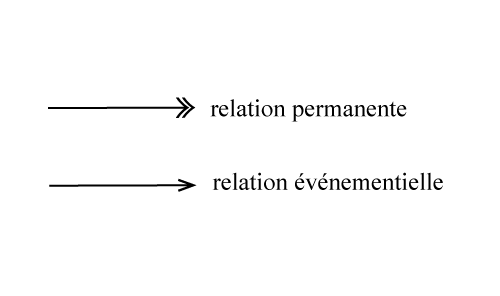
\includegraphics[width=\textwidth]{relation_specification.png}
        \caption{Représentation en spécification}
        \label{fig:relation_specification}
    \end{subfigure}
    \begin{subfigure}[b]{0.4\textwidth}
        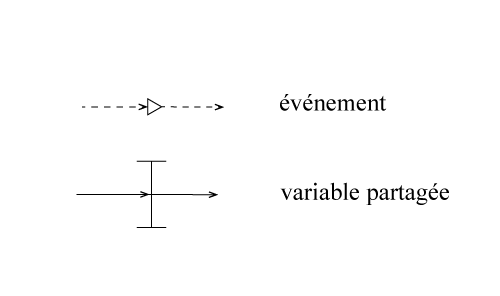
\includegraphics[width=\textwidth]{relation_conception.png}
        \caption{Représentation en conception}
        \label{fig:relation_conception}
    \end{subfigure}
    \caption{Convention de représentation graphique des relations}
    \label{fig:convention_representation_relation}
\end{figure}

\vspace{-1cm}

\begin{figure}[H]
    \centering
    \begin{subfigure}[b]{0.4\textwidth}
        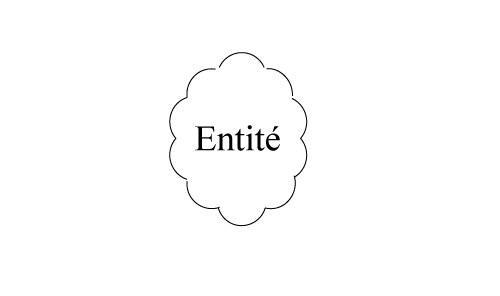
\includegraphics[width=\textwidth]{entite.png}
        \caption{Représentation d'une entité}
        \label{fig:convention_entite}
    \end{subfigure}
    \begin{subfigure}[b]{0.4\textwidth}
        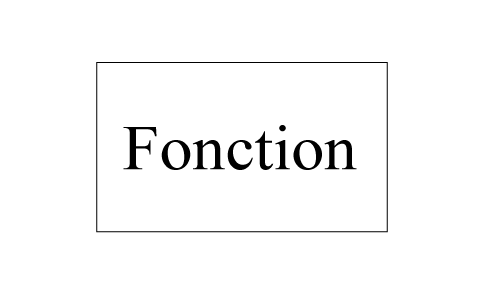
\includegraphics[width=\textwidth]{fonction.png}
        \caption{Représentation d'une fonction}
        \label{fig:convention_fonction}
    \end{subfigure}
    \caption{Convention de représentation graphique des entités et des fonctions}
    \label{fig:convention_representation_entite_fonction}
\end{figure}

\newpage

En ce qui concerne la description de données structurées, les conventions retenues sont les suivantes. Chaque type de structure de données a un nom, un symbole et une syntaxe particulière.

\paragraph{Sélection} ~~\\ \noindent
Ce type est représenté par la figure ci-dessous, par exemple si V est une structure de données de type sélection alors V est défini comme $V=[V_1|V_2|\ldots|V_N]$.

\begin{figure}[H]
    \centering
    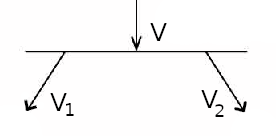
\includegraphics[width=0.3\linewidth]{selection_N_2.png}
    \caption{Notation de la structure de données $V$ de type sélection avec $N=2$}
    \label{fig:selection_N_2}
\end{figure}

\paragraph{Ensemble} ~~\\ \noindent
Ce type est représenté par le symbole suivant. Pour donner un exemple, si V constitue un ensemble alors sa syntaxe est donnée par $V=\{V_1,V_2,\ldots,V_N\}$.

\begin{figure}[H]
    \centering
    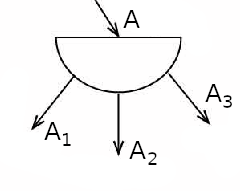
\includegraphics[width=0.25\linewidth]{ensemble_N_3.png}
    \caption{Notation de la structure de données $V$ de type ensemble avec $N=3$}
    \label{fig:ensemble_N_3}
\end{figure}
